\documentclass[11pt,a4paper]{report}
\usepackage[textwidth=37em,vmargin=30mm]{geometry}
\usepackage{calc,xunicode,amsmath,amssymb,paralist,enumitem,tabu,booktabs,datetime2,xeCJK,xeCJKfntef,listings}
\usepackage{tocloft,fancyhdr,tcolorbox,xcolor,graphicx,eso-pic,xltxtra,xelatexemoji}

\newcommand{\envyear}[0]{2025}
\newcommand{\envdatestr}[0]{2025-01-31}
\newcommand{\envfinaldir}[0]{webdb/2025/20250131/final}

\usepackage[hidelinks]{hyperref}
\hypersetup{
    colorlinks=false,
    pdfpagemode=FullScreen,
    pdftitle={Web Digest - \envdatestr}
}

\setlength{\cftbeforechapskip}{10pt}
\renewcommand{\cftchapfont}{\rmfamily\bfseries\large\raggedright}
\setlength{\cftbeforesecskip}{2pt}
\renewcommand{\cftsecfont}{\sffamily\small\raggedright}

\setdefaultleftmargin{2em}{2em}{1em}{1em}{1em}{1em}

\usepackage{xeCJK,xeCJKfntef}
\xeCJKsetup{PunctStyle=plain,RubberPunctSkip=false,CJKglue=\strut\hskip 0pt plus 0.1em minus 0.05em,CJKecglue=\strut\hskip 0.22em plus 0.2em}
\XeTeXlinebreaklocale "zh"
\XeTeXlinebreakskip = 0pt


\setmainfont{Brygada 1918}
\setromanfont{Brygada 1918}
\setsansfont{IBM Plex Sans}
\setmonofont{JetBrains Mono NL}
\setCJKmainfont{Noto Serif CJK SC}
\setCJKromanfont{Noto Serif CJK SC}
\setCJKsansfont{Noto Sans CJK SC}
\setCJKmonofont{Noto Sans CJK SC}

\setlength{\parindent}{0pt}
\setlength{\parskip}{8pt}
\linespread{1.15}

\lstset{
	basicstyle=\ttfamily\footnotesize,
	numbersep=5pt,
	backgroundcolor=\color{black!5},
	showspaces=false,
	showstringspaces=false,
	showtabs=false,
	tabsize=2,
	captionpos=b,
	breaklines=true,
	breakatwhitespace=true,
	breakautoindent=true,
	linewidth=\textwidth
}






\newcommand{\coverpic}[2]{
    % argv: itemurl, authorname
    Cover photo by #2~~(\href{#1}{#1})
}
\newcommand{\makeheader}[0]{
    \begin{titlepage}
        % \newgeometry{hmargin=15mm,tmargin=21mm,bmargin=12mm}
        \begin{center}
            
            \rmfamily\scshape
            \fontspec{BaskervilleF}
            \fontspec{Old Standard}
            \fontsize{59pt}{70pt}\selectfont
            WEB\hfill DIGEST
            
            \vfill
            % \vskip 30pt
            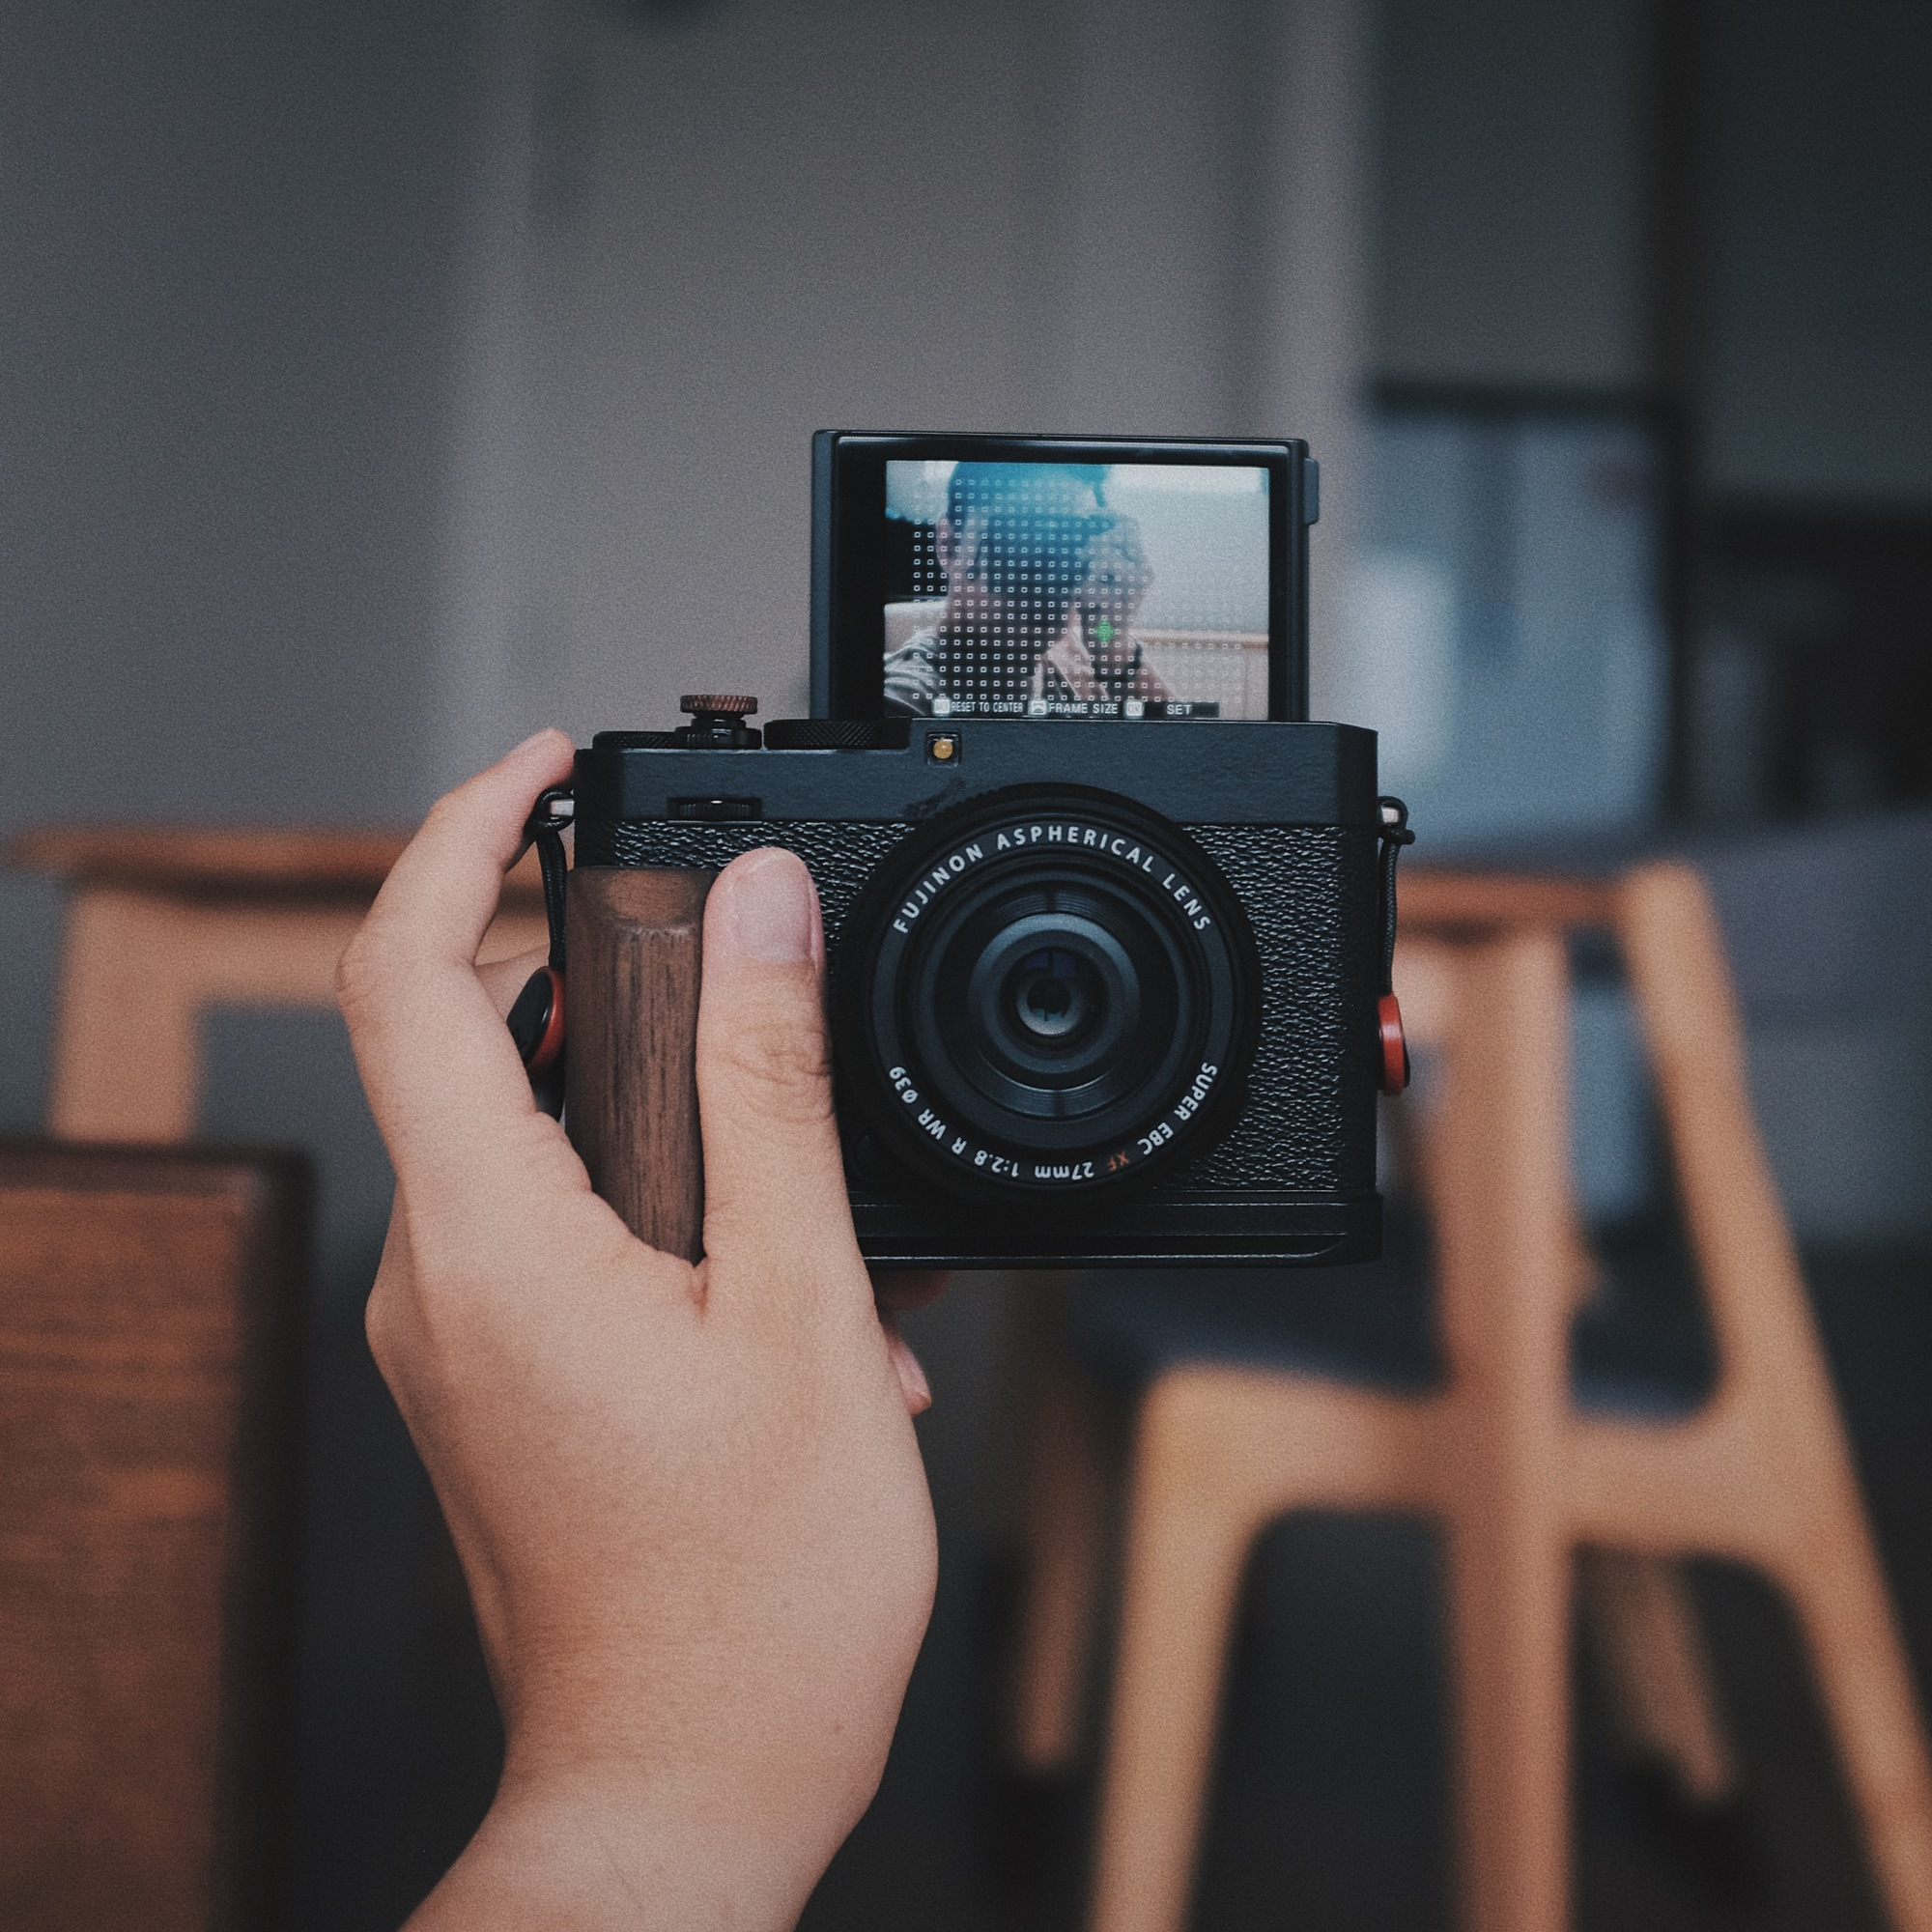
\includegraphics[width=\linewidth]{\envfinaldir/coverpic-prod.jpg}\par
            % \vskip 30pt
            \vfill

            \normalsize\rmfamily\scshape
            \copyright{} The Web Digest Project \hfill\large \envdatestr
        \end{center}
    \end{titlepage}
    % \restoregeometry
}
\newcommand{\simplehref}[1]{%
    \textcolor{blue!80!green}{\href{#1}{#1}}%
}
\renewcommand{\contentsname}{\center\Huge\sffamily\bfseries Contents\par\vskip 20pt}
\newcounter{ipartcounter}
\setcounter{ipartcounter}{0}
\newcommand{\ipart}[1]{
    % \vskip 20pt
    \clearpage
    \stepcounter{ipartcounter}
    \phantomsection
    \addcontentsline{toc}{chapter}{#1}
    % \begin{center}
    %     \Huge
    %     \sffamily\bfseries
    %     #1
    % \end{center}
    % \vskip 20pt plus 7pt
}
\newcounter{ichaptercounter}
\setcounter{ichaptercounter}{0}
\newcommand{\ichapter}[1]{
    % \vskip 20pt
    \clearpage
    \stepcounter{ichaptercounter}
    \phantomsection
    \addcontentsline{toc}{section}{\numberline{\arabic{ichaptercounter}}#1}
    \begin{center}
        \Huge
        \sffamily\bfseries
        #1
    \end{center}
    \vskip 20pt plus 7pt
}
\newcommand{\entrytitlefont}[1]{\subsection*{\raggedright\Large\sffamily\bfseries#1}}
\newcommand{\entryitemGeneric}[2]{
    % argv: title, url
    \parbox{\linewidth}{
        \entrytitlefont{#1}\par\vskip 5pt
        \footnotesize\ttfamily\mdseries
        \simplehref{#2}
    }\vskip 11pt plus 11pt minus 1pt
}
\newcommand{\entryitemGithub}[3]{
    % argv: title, url, desc
    \parbox{\linewidth}{
        \entrytitlefont{#1}\par\vskip 5pt
        \footnotesize\ttfamily\mdseries
        \simplehref{#2}\par\vskip 5pt
        \small\rmfamily\mdseries#3
    }\vskip 11pt plus 11pt minus 1pt
}
\newcommand{\entryitemAp}[3]{
    % argv: title, url, desc
    \parbox{\linewidth}{
        \entrytitlefont{#1}\par\vskip 5pt
        \footnotesize\ttfamily\mdseries
        \simplehref{#2}\par\vskip 5pt
        \small\rmfamily\mdseries#3
    }\vskip 11pt plus 11pt minus 1pt
}
\newcommand{\entryitemHackernews}[3]{
    % argv: title, hnurl, rawurl
    % \parbox{\linewidth}{
    %     \entrytitlefont{#1}\par\vskip 5pt
    %     \footnotesize\ttfamily\mdseries
    %     \simplehref{#3}\par
    %     \textcolor{black!50}{\href{#2}{#2}}
    % }\vskip 11pt plus 11pt minus 1pt
    \begin{minipage}{\linewidth}
            \entrytitlefont{#1}\par\vskip 5pt
            \footnotesize\ttfamily\mdseries
            \simplehref{#3}\par
            \textcolor{black!50}{\href{#2}{#2}}
    \end{minipage}\par\vskip 11pt plus 11pt minus 1pt
}







\begin{document}

\makeheader

\tableofcontents\clearpage




\ipart{Developers}
\ichapter{Hacker News}
\entryitemTwoLinks{Stats – macOS system monitor in your menu bar}{https://news.ycombinator.com/item?id=42881342}{https://github.com/exelban/stats}

\entryitemTwoLinks{California law enforcement misused state databases more than 7k times in 2023}{https://news.ycombinator.com/item?id=42880807}{https://www.eff.org/deeplinks/2025/01/california-police-misused-state-databases-more-7000-times-2023}

\entryitemTwoLinks{Many of the Pokemon playtest cards were likely printed in 2024}{https://news.ycombinator.com/item?id=42880704}{https://www.elitefourum.com/t/many-of-the-pokemon-playtest-cards-were-likely-printed-in-2024/52421}

\entryitemTwoLinks{GitHub Is Down}{https://news.ycombinator.com/item?id=42877995}{https://www.githubstatus.com}

\entryitemTwoLinks{Mistral Small 3}{https://news.ycombinator.com/item?id=42877860}{https://mistral.ai/news/mistral-small-3/}

\entryitemTwoLinks{Antiqua et Nova: Note on the relationship between AI and human intelligence}{https://news.ycombinator.com/item?id=42877709}{https://www.vatican.va/roman\_curia/congregations/cfaith/documents/rc\_ddf\_doc\_20250128\_antiqua-et-nova\_en.html}

\entryitemTwoLinks{Show HN: Audiocube – A 3D DAW for Spatial Audio}{https://news.ycombinator.com/item?id=42877399}{https://www.audiocube.app}

\entryitemTwoLinks{LibreOffice 400M Downloads, and Counting}{https://news.ycombinator.com/item?id=42876998}{https://blog.documentfoundation.org/blog/2025/01/30/400-million-downloads-and-counting/}

\entryitemTwoLinks{Interview with DeepSeek Founder: We're Done Following. It's Time to Lead}{https://news.ycombinator.com/item?id=42876940}{https://thechinaacademy.org/interview-with-deepseek-founder-were-done-following-its-time-to-lead/}

\entryitemTwoLinks{JavaScript Temporal is coming}{https://news.ycombinator.com/item?id=42876840}{https://developer.mozilla.org/en-US/blog/javascript-temporal-is-coming/}

\entryitemTwoLinks{The US government's open data on Data.gov is currently being scrubbed}{https://news.ycombinator.com/item?id=42876055}{https://old.reddit.com/r/climate/comments/1idiliv/the\_us\_governments\_open\_data\_on\_datagov\_is/}

\entryitemTwoLinks{Investigating the case of human nose shape and climate adaptation (2017)}{https://news.ycombinator.com/item?id=42875888}{https://journals.plos.org/plosgenetics/article?id=10.1371/journal.pgen.1006616}

\entryitemTwoLinks{Majority of US teens have lost trust in Big Tech}{https://news.ycombinator.com/item?id=42875399}{https://techcrunch.com/2025/01/29/report-majority-of-u-s-teens-have-lost-trust-in-big-tech/}

\entryitemTwoLinks{PCBs, copper pours, ground planes, and you}{https://news.ycombinator.com/item?id=42874885}{https://lcamtuf.substack.com/p/pcbs-ground-planes-and-you}

\entryitemTwoLinks{Hard Mode Rust (2022)}{https://news.ycombinator.com/item?id=42874605}{https://matklad.github.io/2022/10/06/hard-mode-rust.html}

\entryitemTwoLinks{Commercial jet collides with Black Hawk helicopter near Reagan airport}{https://news.ycombinator.com/item?id=42874301}{https://www.mediaite.com/news/breaking-commercial-jet-collides-with-police-chopper-near-reagan-airport/}

\entryitemTwoLinks{Decompiling 2024: A Year of Resurgance in Decompilation Research}{https://news.ycombinator.com/item?id=42873825}{https://mahaloz.re/dec-progress-2024}

\entryitemTwoLinks{Younger cannabis users have reduced brain function, finds largest study yet}{https://news.ycombinator.com/item?id=42873697}{https://newatlas.com/brain/young-adult-cannabis-brain-function/}

\entryitemTwoLinks{Mathesar – an intutive spreadsheet-like interface to Postgres data}{https://news.ycombinator.com/item?id=42873312}{https://github.com/mathesar-foundation/mathesar}

\entryitemTwoLinks{Blueskyfeedbot: Post RSS Feeds to Bluesky via GitHub Actions}{https://news.ycombinator.com/item?id=42873153}{https://github.com/marketplace/actions/feed-to-bluesky}\ichapter{Phoronix}
\entryitemGeneric{\hskip 0pt{}NVIDIA GeForce RTX 5080 / RTX 5090 Linux Gaming Benchmarks}{https://www.phoronix.com/review/nvidia-rtx5080-rtx5090-linux}

\entryitemGeneric{\hskip 0pt{}Bcachefs Lands More Bug Fixes In Linux 6.14}{https://www.phoronix.com/news/Linux-6.14-Bcachefs-Fixes}

\entryitemGeneric{\hskip 0pt{}Intel Details Its Pluton-Capable Partner Security Engine With Core Ultra Series 2}{https://www.phoronix.com/news/Intel-Partner-Security-Engine}

\entryitemGeneric{\hskip 0pt{}GNOME Display Control Utility "gdctl" Merged For GNOME 48}{https://www.phoronix.com/news/GNOME-Display-Control-gdctl}

\entryitemGeneric{\hskip 0pt{}Yandex Open-Sources Perforator: Find Code Inefficiencies \& "Save Billions of Dollars"}{https://www.phoronix.com/news/Yandex-Open-Source-Perforator}

\entryitemGeneric{\hskip 0pt{}Linux's Sole Wireless/WiFi Driver Maintainer Is Stepping Down}{https://www.phoronix.com/news/Linux-Wireless-Maintainer-2025}

\entryitemGeneric{\hskip 0pt{}NVIDIA 570.86.16 Beta Linux Driver Published With GeForce RTX 5080 / RTX 5090 Support}{https://www.phoronix.com/news/NVIDIA-570.86.16-Linux-Driver}

\entryitemGeneric{\hskip 0pt{}AMD AE4DMA Driver Merged For Linux 6.14}{https://www.phoronix.com/news/Linux-6.14-DMA-AMD-AE4DMA}

\entryitemGeneric{\hskip 0pt{}Intel Linux Graphics Driver Merges "Major Improvement" For Xe3 With VRT Support}{https://www.phoronix.com/news/Intel-Mesa-Xe3-VRT-Merged}


\ipart{Developers~~~~(zh-Hans)}
\ichapter{Solidot}
\entryitemGeneric{\hskip 0pt{}美国版权局称 AI 辅助作品如果包含足够的人类创意可获得版权保护}{https://www.solidot.org/story?sid=80451}

\entryitemGeneric{\hskip 0pt{}LibreOffice 下载量突破 4 亿}{https://www.solidot.org/story?sid=80450}

\entryitemGeneric{\hskip 0pt{}Debian 项目停止在 X 上发推}{https://www.solidot.org/story?sid=80449}

\entryitemGeneric{\hskip 0pt{}Douglas Engelbart 诞辰 100 周年}{https://www.solidot.org/story?sid=80448}

\entryitemGeneric{\hskip 0pt{}Meta 短暂禁止用户发表任何涉及 Linux 的帖子}{https://www.solidot.org/story?sid=80447}

\entryitemGeneric{\hskip 0pt{}腾讯游戏《三角洲行动》被发现会修改用户 CPU 调度和性能释放策略}{https://www.solidot.org/story?sid=80446}

\entryitemGeneric{\hskip 0pt{}心脏病是美国的第一死因}{https://www.solidot.org/story?sid=80445}

\entryitemGeneric{\hskip 0pt{}公共图书馆能给人们的生活带来积极影响}{https://www.solidot.org/story?sid=80444}

\entryitemGeneric{\hskip 0pt{}研究估计到 2100 年欧洲高温死亡人数增加五成}{https://www.solidot.org/story?sid=80443}

\entryitemGeneric{\hskip 0pt{}Google 开源 Pebble 智能手表操作系统}{https://www.solidot.org/story?sid=80442}

\entryitemGeneric{\hskip 0pt{}用开源方法复现 DeepSeek-R1}{https://www.solidot.org/story?sid=80441}\ichapter{V2EX}
\entryitemGeneric{\hskip 0pt{}[Google] Gemini 是否违反了 GDPR?}{https://www.v2ex.com/t/1108370}

\entryitemGeneric{\hskip 0pt{}[分享创造] deepseek.diy}{https://www.v2ex.com/t/1108369}

\entryitemGeneric{\hskip 0pt{}[Android] 一加 Ace5Pro 到了, 5Ghz WiFi 支持 33dBm}{https://www.v2ex.com/t/1108368}

\entryitemGeneric{\hskip 0pt{}[问与答] 二手机械硬盘被回收后有什么用?}{https://www.v2ex.com/t/1108367}

\entryitemGeneric{\hskip 0pt{}[宽带症候群] 有没有用过爱快 Q3000 当 AP 的小伙伴}{https://www.v2ex.com/t/1108366}

\entryitemGeneric{\hskip 0pt{}[奇思妙想] 像 DeepSeek 这种资源要求比较低的大模型有没有可能在工业 AI 中应用?目前工业领域的 AI 一般是什么样的?}{https://www.v2ex.com/t/1108365}

\entryitemGeneric{\hskip 0pt{}[问与答] 国行苹果 15Pro/16Pro 支持 Esim?}{https://www.v2ex.com/t/1108364}

\entryitemGeneric{\hskip 0pt{}[Oracle] oracle 直接把我账号给删了}{https://www.v2ex.com/t/1108363}

\entryitemGeneric{\hskip 0pt{}[宽带症候群] 上海电信 CCTV4K HDR 组播地址分享}{https://www.v2ex.com/t/1108362}

\entryitemGeneric{\hskip 0pt{}[全球工单系统] Github 访问不了?}{https://www.v2ex.com/t/1108360}

\entryitemGeneric{\hskip 0pt{}[问与答] 什么时候出新 12 寸 MacBook}{https://www.v2ex.com/t/1108359}

\entryitemGeneric{\hskip 0pt{}[上海] 从 28 号早上 8 点从魔都出发开车,直到今天 30 号下午 18 点才抵达弥勒。}{https://www.v2ex.com/t/1108357}

\entryitemGeneric{\hskip 0pt{}[MacBook] 新手 Mac 选购}{https://www.v2ex.com/t/1108356}

\entryitemGeneric{\hskip 0pt{}[问与答] 有没有和我一样经常听同一首音乐?}{https://www.v2ex.com/t/1108355}

\entryitemGeneric{\hskip 0pt{}[生活] 今年过年大家观察到身边有哪些变化?}{https://www.v2ex.com/t/1108352}

\entryitemGeneric{\hskip 0pt{}[问与答] 求助新手用 deepseek 写了个类似某博的图片上传发文功能}{https://www.v2ex.com/t/1108350}

\entryitemGeneric{\hskip 0pt{}[问与答] 智行软件提交订单你就是直接帮我候补?}{https://www.v2ex.com/t/1108349}

\entryitemGeneric{\hskip 0pt{}[MacBook Pro] 现在买 m1 pro 还是 m3pro}{https://www.v2ex.com/t/1108348}

\entryitemGeneric{\hskip 0pt{}[创业组队] 单片机开发需求}{https://www.v2ex.com/t/1108347}

\entryitemGeneric{\hskip 0pt{}[地球] 广东的朋友春节都在干什么?}{https://www.v2ex.com/t/1108344}

\entryitemGeneric{\hskip 0pt{}[微软] Copilot+ PC 已经可以本地运行 DeepSeek R1 模型}{https://www.v2ex.com/t/1108343}

\entryitemGeneric{\hskip 0pt{}[问与答] [餐刻 App] 3.0 版}{https://www.v2ex.com/t/1108342}

\entryitemGeneric{\hskip 0pt{}[问与答] 试管和工作之间选哪个,表示很纠结,真的不知道咋办了}{https://www.v2ex.com/t/1108340}

\entryitemGeneric{\hskip 0pt{}[酷工作] 郑州,长沙,重庆年后找工作的看过来。}{https://www.v2ex.com/t/1108339}

\entryitemGeneric{\hskip 0pt{}[问与答] 怎么快速制作聊天表情包?}{https://www.v2ex.com/t/1108337}

\entryitemGeneric{\hskip 0pt{}[问与答] 网易云 MP3 格式格式上传云盘, 还会吞掉部分 是咋回事呢?}{https://www.v2ex.com/t/1108336}

\entryitemGeneric{\hskip 0pt{}[生活] 春节期间给大家分享几个跟``酒''这个话题有关的视频。}{https://www.v2ex.com/t/1108335}

\entryitemGeneric{\hskip 0pt{}[香港] 没有之前工作经验的数字游民去香港开户怎么安排?}{https://www.v2ex.com/t/1108334}

\entryitemGeneric{\hskip 0pt{}[问与答] 问一个大模型本地部署的问题}{https://www.v2ex.com/t/1108333}

\entryitemGeneric{\hskip 0pt{}[问与答] 好像最近 Deepseek 的网络不太稳定}{https://www.v2ex.com/t/1108331}

\entryitemGeneric{\hskip 0pt{}[程序员] 前后端开发毕设,求建议}{https://www.v2ex.com/t/1108330}

\entryitemGeneric{\hskip 0pt{}[奇思妙想] 有没有出租 deepseek 本地模型的云服务器?}{https://www.v2ex.com/t/1108328}

\entryitemGeneric{\hskip 0pt{}[程序员] 可以讲下你看到的编程语言的美吗?}{https://www.v2ex.com/t/1108327}

\entryitemGeneric{\hskip 0pt{}[Chrome] Chorme 老是将首页快捷图标从双列改成单列}{https://www.v2ex.com/t/1108326}

\entryitemGeneric{\hskip 0pt{}[Google] google 的 gemini-2.0-flash-thinking 这个推理模型是不让用了吗}{https://www.v2ex.com/t/1108325}

\entryitemGeneric{\hskip 0pt{}[问与答] x 是什么勾八算法,打开全是 deepseek。}{https://www.v2ex.com/t/1108324}

\entryitemGeneric{\hskip 0pt{}[问与答] 有什么方便老人使用的大模型语音交互小家电吗?}{https://www.v2ex.com/t/1108322}

\entryitemGeneric{\hskip 0pt{}[问与答] 大家有没有整天都犯困的感觉,有没有好的解决办法}{https://www.v2ex.com/t/1108320}

\entryitemGeneric{\hskip 0pt{}[宽带症候群] 二十年前的北網通,南電信,鐵通鐵定不通又回來了?}{https://www.v2ex.com/t/1108318}

\entryitemGeneric{\hskip 0pt{}[ WATCH] Apple Watch 如何让特定联系人电话不震动}{https://www.v2ex.com/t/1108316}

\entryitemGeneric{\hskip 0pt{}[Apple] Macos 15.2 中如何消除``Bartender 5 正在访问你的屏幕''弹窗}{https://www.v2ex.com/t/1108313}

\entryitemGeneric{\hskip 0pt{}[Apple] Apple 日区 ID 没有办法使用国内和香港的 JCB 卡绑定了}{https://www.v2ex.com/t/1108312}

\entryitemGeneric{\hskip 0pt{}[分享发现] 从头搭建一个中国传统文学网站}{https://www.v2ex.com/t/1108311}

\entryitemGeneric{\hskip 0pt{}[VPS] 测评: DMIT-LAX.EB.Intro 29.9-电信联通 9929,移动 CMIN2}{https://www.v2ex.com/t/1108310}

\entryitemGeneric{\hskip 0pt{}[PHP] 国内 PHP 卷王是鸟哥}{https://www.v2ex.com/t/1108309}

\entryitemGeneric{\hskip 0pt{}[游戏] 最近研究出来一套乞丐客厅游戏解决方案}{https://www.v2ex.com/t/1108308}

\entryitemGeneric{\hskip 0pt{}[VMware] 2025 年 ESXi vs Proxmox VE (PVE):虚拟化方案选哪个?}{https://www.v2ex.com/t/1108307}

\entryitemGeneric{\hskip 0pt{}[JavaScript] 求前端大佬解惑, HTML 里的文本怎么做逐行滚动?}{https://www.v2ex.com/t/1108305}

\entryitemGeneric{\hskip 0pt{}[Android] 有没有什么开源(可定制)的,类似 VMOS 的 Android in APK 方案}{https://www.v2ex.com/t/1108304}

\entryitemGeneric{\hskip 0pt{}[程序员] VMware Unity 替代品求推荐!}{https://www.v2ex.com/t/1108301}


\ipart{Generic News}
\ichapter{联合早报}
\entryitemWithDescription{沈泽玮:台湾冲突阻遏法案只叫不咬?}{https://www.zaobao.com/news/china/story20240918-4758889}{美国众议院9月9日开启了长达一星期的``中国周'',共通过25项主要涉华法案。(法新社) 美国众议院在当地时间9月9日开启了长达一星期的``中国周'',在美国总统和国会选举举行之前,密集表决数十项与中国有关的法案,共通过25项主要涉华法案……}

\entryitemWithDescription{欧盟电动车关税投票倒计时 中国在分歧中寻支持}{https://www.zaobao.com/news/china/story20240917-4758953}{欧盟27个成员国将于9月25日就是否继续对进口自中国的电动汽车额外征税进行最后表决。图为上海港等待装运出口的电动汽车。(彭博社) 欧盟对中国电动汽车加征关税的投票进入倒计时,正在欧洲访问的中国商务部部长王文涛与欧盟多国政府高层就此进行协商,试图在立场分歧的成员国中争取到更多支持。 受访学者研判,欧盟对中国电动汽车加征关税不可避免,但具体的加税方式和幅度仍有一定弹性,这是王文涛此行与各国谈判的重点……}

\entryitemWithDescription{港府今年将举办逾400项国庆活动}{https://www.zaobao.com/news/china/story20240917-4759341}{再过十多天就是中国国庆75周年,香港天星小轮展示``国庆75周年''\,``三天免费搭小轮''等标语迎国庆。(中新社) 再过十多天就是中国国庆75周年,香港特区政府今年将举办逾400项庆祝活动,希望通过一连串活动庆祝国庆,并且弘扬爱国主义教育及刺激消费。 港府星期二(9月17日)召开记者会,介绍各项庆祝国庆活动和特别优惠,涉及出行及吃喝玩乐等领域……}

\entryitemWithDescription{美空军部长:中国大陆军演精密化 为入侵封锁台湾做准备}{https://www.zaobao.com/news/china/story20240917-4759407}{美国空军部长肯德尔星期一(9月16日)在空军暨太空军协会的一场大会上致辞,提到中国对印太地区日益增长的威胁。(取自美国国防部网站) (华盛顿综合讯)美国空军部长肯德尔指,中国大陆军演的规模越来越大,也更加精密化,这是在专门为入侵、封锁台湾做准备。他也称,中国对印太地区的威胁现在已存在……}

\entryitemWithDescription{批准潜在对台备件军售案后 美派巡逻机过航台海}{https://www.zaobao.com/news/china/story20240917-4758770}{台军士兵8月26日在屏东县枋山训练场进行实弹演习时,从M1167 TOW运载车上发射一枚美制TOW-2A线导反坦克导弹。(路透社) (华盛顿/台北/北京综合讯)在批准潜在对台备件军售案之后,美国派遣反潜巡逻机过航台湾海峡,中国人民解放军东部战区则组织战机跟监美机,并誓言``坚决捍卫国家主权''……}

\entryitemWithDescription{李家超:若香港驻美经贸办被关 受害的是美企}{https://www.zaobao.com/news/china/story20240917-4758797}{香港特首李家超星期一(9月17日)警告,如果美国通过法案,导致香港驻美经贸办关闭,受害的是美国企业。图为李家超9月11日在``一带一路''高峰论坛上致辞。(彭博社) (香港综合讯)香港特首李家超警告,如果美国通过法案,导致香港驻美经贸办关闭,受害的是美国企业。 美国众议院上周通过《香港经济贸易办事处认证法案》,如果参议院也表决通过并交由总统签署成法,香港三个驻美国的经贸办可能将被强制关闭……}

\entryitemWithDescription{美国指中国航空工业集团员工企图实施黑客攻击}{https://www.zaobao.com/news/china/story20240917-4757988}{(华盛顿综合讯)中国航空航天巨头中国航空工业集团一名员工被指试图对美国宇航局、美国军方和其他目标展开黑客攻击。 据彭博社报道,美国检察官布坎南星期一(9月16日)在起诉书中,指控中国航空工业集团39岁的工程师吴宋(音译,Song Wu)企图从美国宇航局、空军、陆军和海军,以及联邦航空管理局取得电脑软件和源代码……}

\entryitemWithDescription{【东谈西论】恒大账务造假 普华永道是共犯还是被拖累?}{https://www.zaobao.com/news/china/story20240917-4756452}{因涉及恒大地产审计项目的违法行为,普华永道中国9月13日被中国财政部和证监会处以4.41亿人民币罚款并被令停业六个月, 广州分所被撤销……}

\entryitemWithDescription{戴庆成:香港输入人才计划大检阅}{https://www.zaobao.com/news/china/story20240917-4744978}{香港于2022年底推出高端人才通行证计划。(法新社) 2019年香港反修例风波过后,数以十万计港人移居海外,令香港出现人才荒。港府为了解决这个问题,在过去几年积极引入``新血'',当中以高才通计划最受瞩目,社会上也不时热议其成效。 高才通全称为高端人才通行证计划,于2022年底推出,申请人年收入须达到250万港元(约42万新元)以上,或本科毕业于全球百强大学并满足一定工作年限等……}

\entryitemWithDescription{中美希望稳定双边关系 中小国家可​​​搭建桥梁}{https://www.zaobao.com/news/china/story20240917-4745091}{中美元首去年11月在旧金山会晤后,双方都希望稳定两国关系,我国巡回大使陈庆珠认为,如果中美两国都认为走向战争不符合它们的利益,那么中小国家就可以做点什么,为双方搭建桥梁。 陈庆珠星期一(9月16日)在李光耀公共政策学院的一场研讨会上说,中国与西方的关系面对诸多困难,有中国智库表示,希望新加坡能协助在中美之间建立更多对话,``因为新加坡受美国信任,也在中国有渠道''……}

\entryitemWithDescription{陈庆珠:世界经历了三次``中国冲击'' 中美的主导力之争将继续}{https://www.zaobao.com/news/china/story20240917-4744996}{李光耀公共政策学院``思想之节庆''的一场研讨会,讨论``历史终结时的中国冲击''。左起是我国巡回大使陈庆珠、通商中国主席李奕贤、李光耀公共政策学院国际关系助理教授何莉菁、李光耀公共政策学院院长柯成兴……}

\entryitemWithDescription{上海遭遇75年来最强台风 扰乱民众中秋假期出行}{https://www.zaobao.com/news/china/story20240916-4745224}{台风贝碧嘉星期一(9月16日)登陆上海,维护人员星期一下午在衡山路上处理倒伏的树木。 (新华社) 台风造成上海上万株数目倒伏或折断。图为一棵倒下的大树砸坏一旁的建筑。(法新社) 台风贝碧嘉登陆上海后,黄浦江苏州河口潮位上涨,乌云密布。(中新社) 中国上海市星期一(9月16日)遭遇75年来最强台风``贝碧嘉''登陆,也是上海有记录以来首次有强台风侵袭……}

\entryitemWithDescription{陆男频长驱偷渡台湾在测试边防实力?}{https://www.zaobao.com/news/china/story20240916-4745161}{中国大陆一名王姓男子在中秋节前夕,乘橡皮艇从浙江宁波抵达台湾新北市林口,主动打电话投案,海巡署人员前去接他上岸。(自由時報) 中国大陆一名王姓男子划橡皮艇于上星期六清晨偷渡到台湾,隔天被新北市地方法院裁定羁押禁见。这是6月以来第二起大陆人士偷渡至台湾,此间专家质疑是否为海防破口,并怀疑对岸是否在测试台湾的边防实力……}

\entryitemWithDescription{中美时隔八月举行国防部工作会晤}{https://www.zaobao.com/news/china/story20240916-4745025}{(北京/华盛顿综合讯)中美双方上周末举行国防部工作会晤;美国官员称,美国积极进行美中两军外交活动,不代表美国对有关中国议题的处理方式发生任何改变。 据中国国防部星期天(15日)晚上通报,北京香山论坛结束后,第18次中美国防部工作会晤上星期六至星期天(9月14日至15日)在北京举行……}

\entryitemWithDescription{中国高校今年拟增足球运动本科专业}{https://www.zaobao.com/news/china/story20240916-4744925}{(北京综合讯)为了培养足球专业人才,中国大专学府今年度拟新增足球运动本科专业,以具体落实中国足球改革。 综合人民网和《南方都市报》报道,中国教育部上星期五(9月13日)发布《2024年度普通高等学校本科专业申报材料公示》。根据公示统计,今年度拟新增专业535个,涉及353所高校,其中39所高校新增足球运动专业……}

\entryitemWithDescription{香港23条首案 港男因穿``光时''上衣被定罪}{https://www.zaobao.com/news/china/story20240916-4743439}{(香港综合讯)香港一名无业男子,今年6月因穿印有2019年反修例抗争口号的上衣而被捕。他星期一承认违反煽动意图罪,成为在《维护国家安全条例》(即《香港基本法》第23条)下被定罪的第一人。 综合港媒《星岛日报》和路透社报道,27岁无业男子诸启邦今年6月12日在石门港铁站附近,未能出示身份证供查阅被警方拘捕……}

\entryitemWithDescription{美国务院:中国释放被关押近20年美籍牧师}{https://www.zaobao.com/news/china/story20240916-4744614}{(华盛顿综合电)中国释放被关押近20年的美国籍牧师,显示北京在中美关系的关键时刻展现善意。 综合彭博社、法新社和路透社报道,美国国务院发言人星期天(9月15日)说:``我们欢迎林大卫(音译,David Lin)从中华人民共和国的监狱获释。他已回返美国,这是他近20年来首次与家人见面。'' 林大卫的女儿艾丽斯告诉美国政治新闻网Politico,她的父亲将抵达得克萨斯州的圣安东尼奥……}

\entryitemWithDescription{中国驻泰使馆:近期并未向湄公河下游泄洪}{https://www.zaobao.com/news/china/story20240916-4743917}{(北京讯)泰国西北部的湄公河因洪水泛滥而决堤,中国否认这是中方泄洪所致,并称近来已持续减少云南景洪水电站的出库流量,以助下游地区抗洪。 中国驻泰国大使馆星期日(9月15日)深夜在官方微信公众号发文说,当天又有媒体报道称中国正在向湄公河泄洪,经向中国主管部门核实,使馆再次澄清,为帮助下游地区应对洪灾,中方近来持续稳定和减少景洪水电站出库流量,不可能对下游地区抗洪救灾形成压力……}

\entryitemWithDescription{加入美国储存可靠度评估计划 台湾军方编列预算采购三类型导弹}{https://www.zaobao.com/news/china/story20240916-4743826}{(台北讯)据台媒报道,台湾军方持续向美国采购可简易操作的导弹,预计在2024年、2031年以前获得400枚``标枪''反装甲导弹、2485枚``刺针''人携式防空导弹……}

\entryitemWithDescription{韩咏红:中美分头追逐全球南方}{https://www.zaobao.com/news/china/story20240916-4730719}{9月5日,中国外长王毅(中)同中非合作论坛非方现任共同主席国塞内加尔外长法勒(左)、下任共同主席国刚果外长加科索(右),在北京共同会见中外记者并答问。(路透社) 进入气候宜人的9月,中国接连举行了两场受瞩目的国际会议,一是聚集非洲53国国家元首与政要的中非合作论坛,接着是周末刚闭幕的北京香山论坛。 两场活动的参与者不同,规模也有很大差距……}

\entryitemWithDescription{菲律宾船只撤离中菲争议海域后 将再派船接替}{https://www.zaobao.com/news/china/story20240915-4730494}{这张在9月15日拍摄,并由菲律宾海岸警卫队提供的照片显示,菲律宾海岸警卫队船马格巴努亚号抵达了菲国巴拉望岛的一个港口。菲律宾早前以发现填海活动为由,今年4月派出马格巴努亚号前往萨比纳礁。(法新社/菲律宾海岸警卫队) 菲律宾国家海事委员会星期天(9月15日)发声明称,该国海岸警卫队一艘巡逻舰已离开萨比纳礁争议海域……}

\entryitemWithDescription{台风贝碧嘉直击中国华东 多趟本地与沪杭间航班取消}{https://www.zaobao.com/news/china/story20240915-4730611}{9月15日在上海外滩滨江步道上,一名外籍游客的雨伞被大风吹起。台风贝碧嘉的中心当天下午5时位于上海市东偏南方大约435公里的东海海面上,中心附近最大风力有13级。(中新社) (上海/新加坡综合讯)台风贝碧嘉预计将为中国华东沿海地区带来狂风暴雨,多趟往返新加坡与上海和杭州的航班取消……}






\clearpage
\leavevmode\vfill
\footnotesize

Copyright \copyright{} 2023-2025 Neruthes and other contributors.

This document is published with CC BY-NC-ND 4.0 license.

The entries listed in this newsletter may be copyrighted by their respective creators.

This newsletter is generated by the Web Digest project.

The newsletters are also delivered via Telegram channel \CJKunderline{\href{https://t.me/webdigestchannel}{https://t.me/webdigestchannel}}.\\
RSS feed is available at \CJKunderline{\href{https://webdigest.pages.dev/rss.xml}{https://webdigest.pages.dev/rss.xml}}.

This newsletter is available in PDF at
\CJKunderline{\href{https://webdigest.pages.dev/}{https://webdigest.pages.dev/}}.

The source code being used to generate this newsletter is available at\\
\CJKunderline{\href{https://github.com/neruthes/webdigest}{https://github.com/neruthes/webdigest}}.

This newsletter is also available in
\CJKunderline{\href{http://webdigest.pages.dev/readhtml/\envyear/WebDigest-20250131.html}{HTML}} and
\CJKunderline{\href{https://github.com/neruthes/webdigest/blob/master/markdown/\envyear/WebDigest-20250131.md}{Markdown}}.


\coverpic{https://unsplash.com/photos/a-statue-of-a-person-holding-a-golden-trophy-yUMTuj088PQ}{bharath kumar}


\end{document}
